%% uctest.tex 11/3/94
%% Copyright (C) 1988-2004 Daniel Gildea, BBF, Ethan Munson.
%
% This work may be distributed and/or modified under the
% conditions of the LaTeX Project Public License, either version 1.3
% of this license or (at your option) any later version.
% The latest version of this license is in
%   http://www.latex-project.org/lppl.txt
% and version 1.3 or later is part of all distributions of LaTeX
% version 2003/12/01 or later.
%
% This work has the LPPL maintenance status "maintained".
% 
% The Current Maintainer of this work is Daniel Gildea.

\documentclass[11pt]{ucthesis}
\def\dsp{\def\baselinestretch{2.0}\large\normalsize}
\dsp

\usepackage{graphicx}
 \usepackage{subfigure}% subcaptions for subfigures
 \usepackage{lettrine}% dropped capital at beginning of paragraph
 \usepackage{hyperref}% embedding hyperlinks [must be loaded after dropping]
 \usepackage{amsmath}
 \usepackage{color}
\begin{document}

% Declarations for Front Matter

\title{Modeling and Control of Active Twist Aircraft}
\author{Nicholas Bryan Cramer}
\degreeyear{2017}
\degreemonth{March}
\degree{DOCTOR OF PHILOSOPHY}
\chair{Professor Mircea Teodorescu}
\committeememberone{Professor Ricardo Sanfelice}
\committeemembertwo{Dr. Sean Swei}
\numberofmembers{3} %% (including chair) possible: 3, 4, 5, 6
\deanlineone{Dean Tyrus Miller}
\deanlinetwo{Vice Provost and Dean of Graduate Studies}
\deanlinethree{}
\field{Computer Engineering}
\campus{Santa Cruz}

\begin{frontmatter}

\maketitle
\copyrightpage

\tableofcontents
\listoffigures
\listoftables

\begin{abstract}
Theses have elements.  Isn't that nice?

\end{abstract}

\begin{dedication}
\null\vfil
{\large
\begin{center}
To ,\\\vspace{12pt}

\end{center}}
\vfil\null
\end{dedication}


\begin{acknowledgements}
I want to thank
\end{acknowledgements}

\end{frontmatter}

%%%%%%%%%%%%%%%%%%%%%%%%%%%%%%%%%%%%%%%%%%%%%%%%%%%%%%%%%%%%%%%%%%%%%%%%%%%
\chapter{Introduction}

\section{Motivation}
Demand for commercial air travel has increased at an steady rate of $9\%$ annual growth rate of passenger and freight traffic globally over the past three decades. \cite{upham2003environmental} With the continued increase in demand for air travel the ramifications of air travel must be addressed. These range from health concerns to ever increasing $CO_2$ emissions. It is expected that between 1995 and 2050 the contribution of $CO_2$ from air travel will in increase by a factor of 36 which is why air travel and its efficiency are heavily discussed in climate change policy. \cite{olsthoorn2001carbon} While air travel has it's downsides it is also a critical component for trade \cite{smith2001world}, regional developments \cite{marazzo2010air}, and intercultural communications \cite{adey2007flying}. With air travels critical role in financial and social institutions it is unreasonable to expect that anything less and a holistic solution of technological and policy advancement could appropriately address the salient issues associated with it.

Increased aircraft efficiency is typically achieved either by a reduction of weight or and increase of aerodynamic efficiency. In the industry the most common production level approach is to reduce weight through the use of composites. For example Boeing's 787 Dreamlines which was able to achieve a 20\% weight reduction by using carbon fiber plastic composites. \cite{hale2006boeing} On the other end of the spectrum the aerospace community has been investigating the use of morphing aircraft to increase the aerodynamic efficiency through the use of shape morphing.\cite{barbarino2011review,kuzmina2002review,sofla2010shape} Shape morphing can be described as the ability of an aircraft to change some form of its geometry. There are very few limitation of what can be considered ``shape morphing'' other than the fact that traditional hinged flaps/slats are not sufficient changes in the aircraft geometry to be counted. Figure \ref{fig:airGeo} shows the general range of aircraft geometries that can be adjusted for reference. 

\begin{figure}[h]
\centering
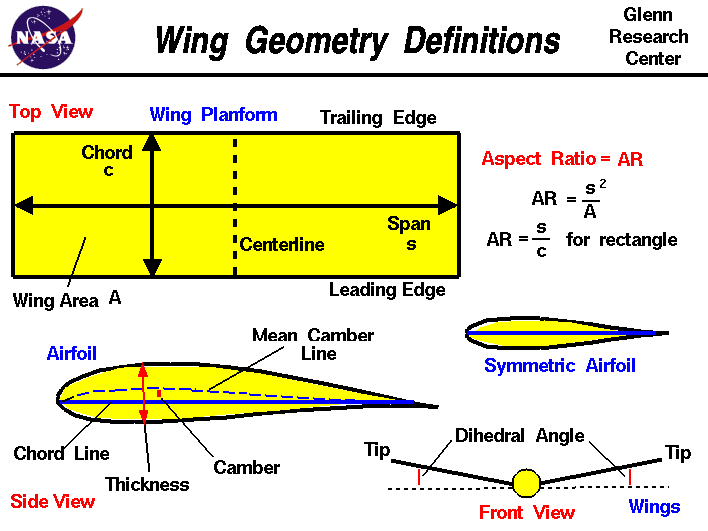
\includegraphics[width=0.75\linewidth]{./Figures/AircraftGeom.png}
\caption{General definitions of aircraft geometries, provided by NASA Glenn Research Center}
\label{fig:airGeo}
\end{figure}

Shape morphing typically achieves the increase in aerodynamic efficiency by changing the aircraft geometry to become more optimal at various flight conditions. Typical fixed wing aircraft are designed to have maximum efficiency around their nominal cruise conditions, which necessarily results in the design being sub-optimal at other flight conditions. In theory the aircraft should spend the vast majority of it's flight time at its nominal cruise condition but due to things like weather, airspace congestion, and distance of flight this is not always true and shape morphing can help address this problem.  

There are four major challenges associated with making shape morphing a viable technology for the industry, distributed high-power density actuation, structural mechanization, flexible skins, and control law development. \cite{reich2007introduction} Of these primary challenges we will be addressing the control law development but the linkage between all of these challenges will be evident. I will specifically be focusing on the development of reasonable models, control and capability analysis of an active twist aircraft. Wing twist is defined as the angle that the wing tip is compared to the angle that the wing meets the aircraft body as shown in Figure \ref{fig:twist}. Wing twist was selected because it is capable of generating many interesting and potentially important phenomena for increased efficiency.

\begin{figure}[h]
\centering
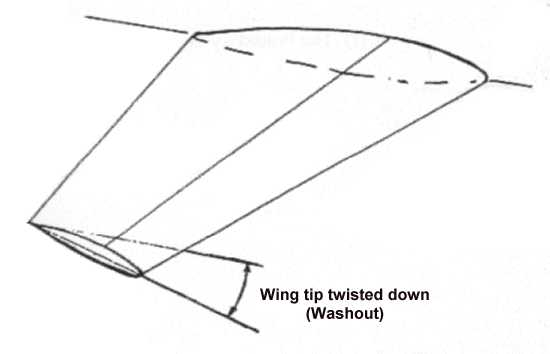
\includegraphics[width=0.75\linewidth]{./Figures/twist.jpg}
\caption{Definition of wing twist, where the tip of the wing is twisted at an angle different than the one that the wing meets the plane body at}
\label{fig:twist}
\end{figure}

\section{Applications}
Our motivation example focused primarily on commercial aircraft but the application space for this research can be broken down into three area, where commercial aircraft are but one part.
\begin{itemize}
\item Commercial Aviation - The commercial aviation sector was touched on above but effective control of active twist could have a direct and immediate impact on this field. A very effective use of wing twist could be the creation of active twisting winglits that can be trimmed to optimal wash out of various flight regimes. This could provide significant performance increases during take-off and landing.
\item Military Aircraft - The military has a desire to have an aircraft that is flexible to a multitude of missions. The use of active twist technology would allow for more efficient vehicles and longer flights but more crucially would increase the performance envelope of the aircraft. It could be especially important as an enabling technology for other high efficiency designs such as blended body and flying wings where the minimum stability margin of the aircraft can be catastrophically affected by the discontinuities that come from traditional flaps.
\item Unmanned Aerial Vehicles (UAVs) - UAVs have a lot of promise as means of delivery or inspection but one of the primary problems is that the rotocopter set-up that is ideal for these missions has sever longevity issues while the fixed wing variant need long ranges to take off and land and are difficult to loiter in the same spot. The active twist technology could help by decreasing the loiter speed and loiter radius of the UAV while also decreasing the range necessary to take off and land.
\item High Altitude Long Endurance (HALE) Aircraft - Active twist for HALE aircraft have many of the same advantages as commercial aviation but they also have a distinct advantage of not typically having passengers. This means that it is possible for the HALE to take advantage of some of the aerodynamic efficiency gains of active that can be seen in flapping flight that would be untenable for passengers.
\end{itemize}

\section{Contributions of this Work}
In this work we try to take a holistic approach to the design and analysis of the active twist controllers as such there are some varied contributions to the field which are listed below.

\begin{itemize}
\item Development of an aeroelastic simulation method that is specifically tailored to the targeted operating regime. 
\item Design of wind tunnel tests to access the broader capabilities of the technology and validate the simulation.
\item Creation of decentralized control expanding on the work of Siljak \cite{siljak2011decentralized} to address the issues associated with overlapping decentralized control.
\item Expansion of the concept of the transfer matrix method as a means of control centered modeling and decentralized structural stabilization.
\item Explored the use of aerodynamic database for structural state estimation and inner loop active twist control.
\end{itemize}

%%%%%%%%%%%%%%%%%%%%%%%%%%%%%%%%%%%%%%%%%%%%%%%%%%%%%%%%%%%%%%%%%%%%%%%%%%%
\chapter{Background}
\section{Aeroelastic Modeling}
\label{sec:aeroMoldLit}

Aeroelasticisity has been a well known and well studied problem sense shortly after the creation of planes.   To date many of the studies use some combination of an aerodynamic simulator that then couples with the mode shapes and the wing. Indeed Nguyen et. al. \cite{nguyencoupled} use an elastic wing model, a vortex lattice program (Vorview), and a geometry modeling tool coupled together to create an aeroelastic model. The elastic wing modeling utilizes twist, flapwise and chordwise bending as well as having the bending-torsion coupled included. The eventually simplify by neglecting the chordwise bending because it is noted that it is small, especially in comparison to the wing sweep angle.

The aeroelastic angle of attack is defined to be the velocity of wind in the chordwise direction over the velocity in the flapwise direction. These velocities are a combination of the air speed and the elastic velocities. The forces resulting from the aeroelastic angle of attack are calculated by using the aeroelastic angle of attack and the lift and pitching moment coefficients as calculated by Vorview.

The static and dynamic analysis were performed by galerkin method to separate the mode shapes for each given natural frequency. The static uses the analysis of the primary mode with no dynamics and is added to the dynamics modes. Each state equation is the result of the summation of a primary set of modes and then the states are converted into the modal coordinates are used for the calculations.

In \cite{nguyen2012aeroelastic} the work from \cite{nguyencoupled} is extended. Nguyen et. al present variable camber continuous trailing edge (VCCTE) flat system to control the wing twist and wing bending in order to shape the wing. The proposed wing would be shaped into the optimal configuration for drag reduction during cruising and possibly lift enhancement during take off. The VCCTE would consist of an three component flap to dynamically shape the the mean chord of the airfoil to change the aerodynamic center location and the spanwise variation in lift.

The generic transport model (GTM) was used as the basis of the rigid body model. The aeroelastic equations were derived for the wings using primarily the adjusted local angle of attack and the lift, drag, and moment coefficients associated with the instantaneous wing configuration. The beam model used was the same that was used in \cite{nguyencoupled} with the addition of bending-torsion coupling and the inclusion of cordwise bending. The GTM has jet engines attached and the affects of the thrust from the engines on the wings was also considered, as was the fact that fuel is stored in the wings resulting in the wing density, area moment of inertia, and the bending torsion constants.

The rigid body mechanics an the aeroelastic equations associated with the wings were coupled via the integration of the local lift, drag and moments along the span. This was important because the frequencies of the aeroelastic and rigid body components are close and coupled. The equations of motion take the form of a time varying state space model. A observer is proposed to estimate the local angle of attack and then a LQR control was proposed to minimize the drag, states and control.

With many of the same assumptions and that Nguyen et. al. work on Wang et. al presented a reduced modal approach to modeling nonlinear aeroelastic responses in flexible wings in \cite{wang2014nonlinear}. They also presented $H_{\infty}$ control for the trim from the reduced modal model. The wing was treated like a typical beam system to get the expected modes then the amplitude of the modes were used to generate that dynamics which was then reduced. The dynamic modal equation relates linearly the natural frequencies to the modal amplitudes and the interaction between the modal amplitudes as well as the external forces.

The aerodynamics forces were calculated using a 2-D unsteady airfoil theory to develop lifting, drag, and moment coefficient with respect to angle of attack. The local angle of attack is generated from the proportion of vertical velocity, resulting velocity from the angular velocity and the total airspeed with the induced angle of attack subtracted. The induced angle of attack was generated with an approximation of Theodorsen's lift deficiency function.

Due to the reduction scheme there can be some drift in the values that must be checked via a spanwise integration. The external force effects due to thrust, gust, and control surface input were converted to the modal coordinates to create the dynamics equation, which were used for the proposed control.

Getting away from the assumed mode shapes that the previous works utilized Su proposed a strain based modeling technique for a slender flexible wing in \cite{su2014modified}. The localized strain components can be integrated to arrive at the local position and positional rate components for the finite elements. To allow for warping of the system a warping field was proposed where a finite selection of warping modes for the cross sectional area and the effects of neighboring warped cross sections are considered. Then using the virtual work concept the external and internal virtual work was combined to derive the equations of motion.

\section{Morphing Wings}
Morphing wings as a means of control is an intuitive and readily understandable means of controlling an aircraft. In our daily life we often see birds flying and their primary mechanism of motion control is changing the shape of their wings. Not surprisingly then the first attempt at roll control was done via wing warping during the Wright brothers first flight. \cite{friswell2009prospects} The use of compliant wing morphing mechanisms quickly fell out of favor it seems likely this was due to the rise of the structural shell mechanism, for which the shell of the aircraft became the primary structural component. While aircrafts still used truss structures like that found in the Wright brother's plane the weight was reduced dramatically by having the shell bare the load. \cite{weisshaar2011aerospace} It seems likely that the additional engineering effort to make the shell compliant to actuation while resisting aeroloading and the relative ease at which traditional control surfaces could be manufactured resulted in the dormancy of morphing wing research.

Work on compliant morphing wings resumed in the 1980's with Air Force Research Laboratory's (AFRL) the Active flexible wing (AFW) technology project that was using traditional control surfaces to shape a compliant wing. \cite{miller1988active} This was eventually followed by the ``PARTI'' \cite{pinkerton1996controlled} and DAPRA's Smart Wing Project \cite{kudva2001overview} who used smart materials as a means of actuation for the morphing airfoil, irreversibly linking the morphing wing research to the continued development of smart materials. With the turn of the century research in morphing aircraft exploded, in the next few sections we will explore some of the more relevant morphing wing research.

\subsection{Camber Morphing}
Changing the camber of an airfoil is probably the most researched area of morphing wing research. This is because the dramatic changes that the camber can have on the aerodynamic performance. 

One of the most successful Small Business Innovation Research (SBIR) in recent memory has been FlexSys which created an variable camber trailing edge for  wings\cite{kota2009mission} and rotors\cite{kota2008adaptive}. The FlexSys system uses a underlying compliant mechanism to control the structural deformation of the airfoil and therefore the camber with a simple rotary actuator. This structure encourages a reduction of stress concentrations  and the weight  of joints while minimizing backlash. The interface between the stiff wing and the compliant trailing edge is an elastomer membrane. FlexSys was able to demonstrate the effectiveness of their variation of the camber morphing through model test flight and are currently performing full scale slight systems both of which have yielded positive results. 

The spiritual successor at AFRL to the ARW program is the AFRL Variable Camber Compliant Wing (VCCW) which shares a lot of similarities to the FlexSys system. The VCCW is focused on optimization of the variable camber design by combining the the leading and trailing edge mechanism, eliminating the need for stretchable skin, while minimizing the energy consumption. The VCCW has been exhaustively studied prior to flight testing via bench top testing and simulations \cite{miller2015fluid} as well as wind tunnel testing \cite{zientarski2015wind} both showing the expected performance increases. 

The final camber morphing project that I will highlight is NASA and Boeing's Variable Camber Continuous Trailing Edge Flap (VCCTEF). The VCCTEF bears some similarities to the AFW project in that it is using the the flaps to control the aerodynamic forces and the resultant wing shaping. This is achieved via numerous trailing edge flaps that changed the airfoil camber and are attached to each other via and elastomer filling. The flap actuation is achieved with a slow large displacement using Shape Memory Alloy (SMA) and faster electric drive motors for the outboard flap.\cite{urnes2013mission} The configuration of the actuator results in actuation constraints that much be taken into account. \cite{swei2014aeroelastic} Of the camber morphing technologies presented here the the VCCTEF project is one of the only ones that committed a significant effort to investigating the control of the aircraft\cite{nguyen2012aeroelastic} though additional validation has not been completed beyond simulations.

\subsection{Flapping Flight}
There has been a large amount of research in the area flapping flight. \cite{shyy2010recent} While the field of flapping flight field is expansive and robust we will be focusing only on the research relevant to this thesis in this section. The work relating to relevant modeling techniques are highlighted in Section \ref{sec:aeroMoldLit}. 

Much of the flapping flight research has been focused on creating bio-mimetic devices to study the flight characteristics of flying animals. A group from the Department of Integrative Biology at the University of California Berkeley, has created an dynamically scaled model of a common fruit fly's wing to study the effects of different patterns of wing strokes. They were able to show that the wing twist during the stroking motion can result in rotational circulation that they theorized can be used as a means of directional control and force modulation.\cite{dickinson1999wing} In later works they were able to show that the wing twist had a significant impact on the lift force in flight, especially when the wing strokes are of small amplitudes. They also showed that the quasi-steady estimates was limited in its capability of replicating the kinematic patterns,\cite{sane2001control} while continuing to expand on the means of quasi-static simulation techniques.\cite{sane2002aerodynamic}

There is on going work at AFRL into the control of flapping micro aerial vehicles. Much of the work has focused on the use of split-cycle control to achieve various maneuvers. \cite{weintraub2014implementation} Split-cycle control is at it's core using asymmetric cosine waves as show in Figure \ref{fig:splitCycle}, where the period and phase of the rising and falling edge are modulated to create asymmetric forces inducing 6 dof of control. The  work has been focused primarily on creating biomimetic hovering. \cite{doman2010wingbeat,oppenheimer2011dynamics}

\begin{figure}[h]
\centering
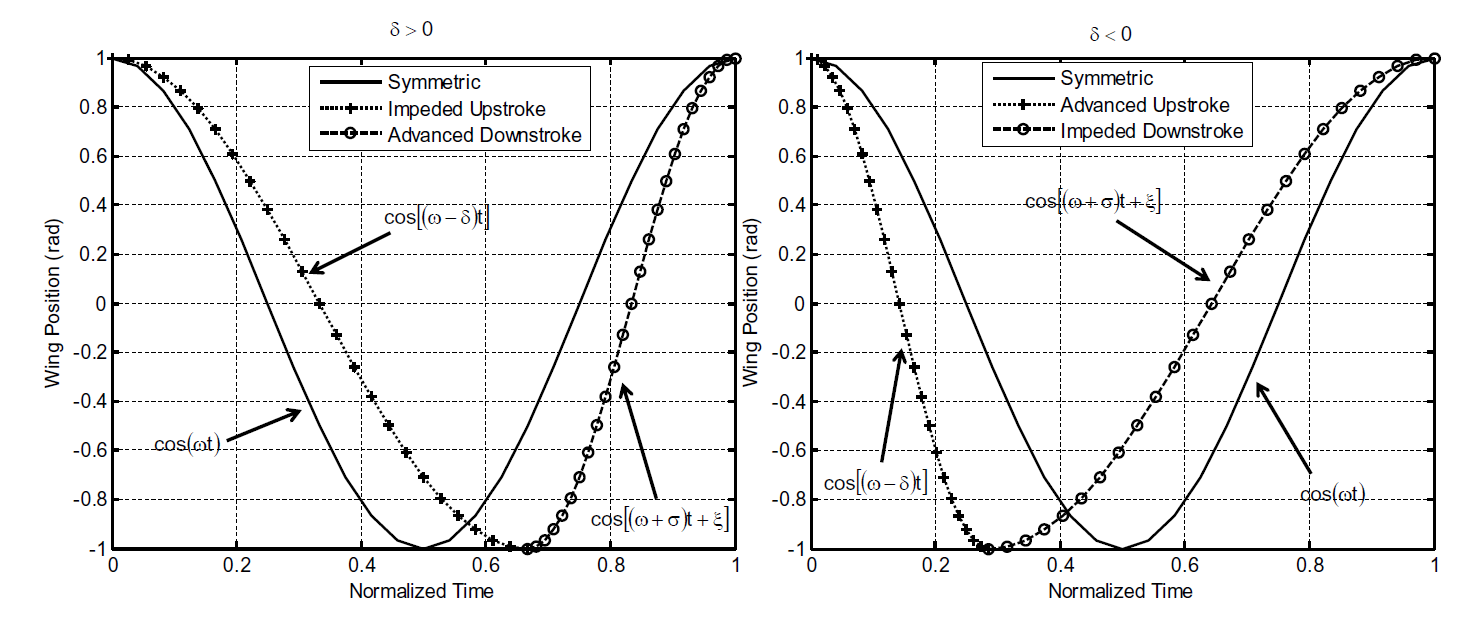
\includegraphics[width=1\linewidth]{./Figures/splitCycle.png}
\caption{Split-cycle example waveform. Figure taken from  \cite{weintraub2014implementation}.}
\label{fig:splitCycle}
\end{figure}

\subsection{Active Twist}

The research in the thesis is focused on the modeling and control of active twist aircraft making the work presented in this section of critical importance. To the authors knowledge the first known modern investigation of variable twist on a wing was performed by Ferris at NASA Langely. \cite{ferris1977wind} Ferris created an model aircraft with $35^{o}$ sweep and the ability to modulate the camber of the leading and trailing edge as well as the sectional twists. In this study the twist was implemented by having the leading edge camber morphing hinge being more swept than the trailing edge. As a result of the implementation the variable twist the affects of the twist and camber changed could not really be de-coupled and as a result only the camber was investigated.

Unlike the morphing wing field in general investigation into specific active twist technology did not begin until the mid 2000's. This is likely because the flexibility that camber morphing offers over active twist. Camber also has an conceptual advantage because modern aircraft's aileron, flaps, and slats are generally intended to replicate variable camber. Keeping that in mind much of the research that was done on active twist has been part of the creation of a fully adaptable aircraft. This is the case for \cite{neal2004design} where Neal \textit{et. al.} created a fully adaptive aircraft that was able to change it's span, sweep and tip twist. While they had created an aircraft that was capable of active tip twist when they performed the wind tunnel testing they did not report any of the results from the tip twist focusing instead on the mechanisms that would have the largest most immediate affects on lift like variable span.

One of the only studies of active twist technology that was actually flown was by Abdulrahim \textit{et. al.} \cite{abdulrahim2004flight}. They made two different small sized UAV's one with wing curling capabilities and one with wing twisting capabilities they flew both and compared the two aircraft performance. The aircraft wings are not of a typical NACA airfoil like design, instead they are more akin to reinforced membranes. The authors noted that it was difficult to achieve system identification of the curling aircraft due to time0varying asymmetries, limited data collection and data quality. They did not attempt to perform the molding on the wing twisting aircraft but it seems likely that the last two issues remained as well. They were able to show that the wing twist was an effective means of roll control.

Of the previous active twist research the most relevant to the work presented in this thesis is the work of Majji \textit{et. al.}\cite{majji2007design} at Texas A\&M and the later work of Vos \textit{et. al.}\cite{vos2010mechanism} at Delft University of Technology. Majji \textit{et. al.} developed an redundant torque tube active twist set-up where the wing box was split into one third sections with a telescoping torque rod in attaching in four places to allow for multiple combinations of twist. The wing box and torque tube was then skinned using an elastomeric skin. They used Prandtl's lifting line theory as a means to calculated the expected lift coefficient and compare it to the wind tunnel results. They noted in the paper that there were some structural issues with the design, primarily the skin ballooned and dimpled to the point that it was necessary to compensate for those issues in the calculations. They were still able to show the ability to control the lift coefficient with each twist location with the root twist location having the largest affect.

Vos \textit{et. al.}\cite{vos2010mechanism} set out to address some of the more common issues with active twist technology as were seen in \cite{majji2007design}. The basic premise was that the traditional wing box is not an effective means of inducing twist but that instead the outer shell can be viewed as a torque tube itself and the skin could be addressed by allowing the an open tube but with a control mechanism to help with the modulation of the torsional stiffness. They achieved their goal with a clever threaded rod system attached at the trailing edge of the carbon fiber reinforced skin and allowing the skin to slide freely on the ribs which could rotate freely on the spar. For modeling purposes they used both lifting line and vortex lattice code and then compared the results to wind tunnel tests. They found that the models matched the wind tunnel test relatively well especially at higher angles of attack where the lift induced drag would dominate. 

%\section{Control}
%\subsection{Aeroelastic Control}
%\subsection{Decentralized Control}

%%%%%%%%%%%%%%%%%%%%%%%%%%%%%%%%%%%%%%%%%%%%%%%%%%%%%%%%%%%%%%%%%%%%%%%%%%%
\chapter{Modeling}
The appropriate modeling of the active twist wing is critical to further exploration on the capabilities of active twist. Due to the nature of active twist the structure becomes inherently aeroelastic. Aeroelasticity is the coupling of the aerodynamics, the rigid body dynamics of the aircraft, as well as the structural dynamics primarily of the wings. A conceptual diagram of this interaction can be seen in Figure \ref{fig:AEDiag}. The nature of aeroelasticy requires the development of both the structural modeling aspects and aerodynamic modeling with a special focus on the combination of the two.

\begin{figure}[h]
\centering
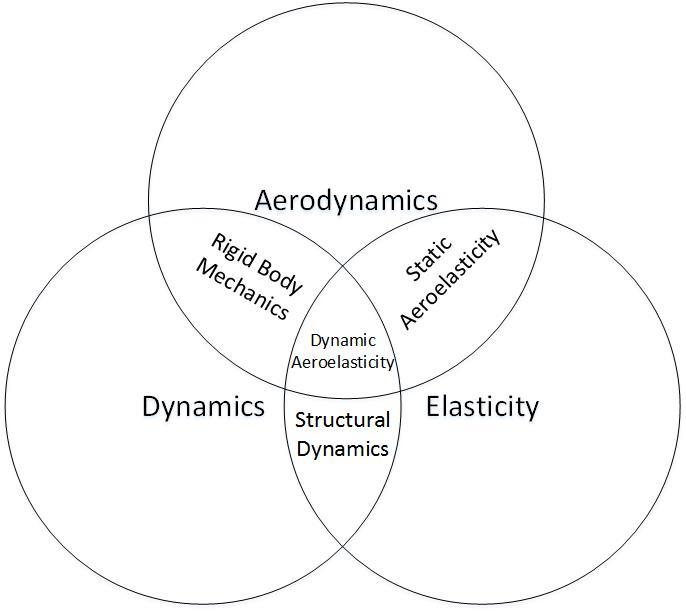
\includegraphics[width=0.4\linewidth]{Figures/AeroelasticConceptDiagram.jpg}
\caption{Conceptual diagram of the aeroelastic field. This figure is a recreation from \cite{hodges2011introduction}}
\label{fig:AEDiag} 
\end{figure}

\section{Structural Modeling}
One of the primary components of aeroelastic modeling is the structural modeling that will be coupled with the aerodynamics. I used the Galerkin finite element method (GFEM) to model the wing. The GFEM is presented in \cite{fertis1999nonlinear} the basic approach to GFEM is to use a assumed shape that takes a basic spline and use the energetic equations to populate the mass and stiffness matrix. For a standard beam bending scenario that we will be eventually extending to a wing structure a hermite cubic spline was used resulting in the assumed shape in Equation \ref{eqn:hCube}.
\large
\begin{eqnarray}
	\begin{array}{ll}
		w(x) = f_1(x)w_i +f_2(x)\phi_i+f_2(x)w_{i+1}+f_2(x)\phi_{i+1}\\
		f_1(x) = 1-\frac{3x^2}{l_i^2}+\frac{2x^3}{l_i^3}\\
		f_2(x) = x-\frac{2x^2}{l_i}+\frac{x^3}{l_i^2}\\
		f_3(x) = \frac{3x^2}{l_i^2}-\frac{2x^3}{l_i^3}\\
		f_4(x) = \frac{-x^2}{l_i}+\frac{x^3}{l_i^2}
	\end{array}
\label{eqn:hCube}
\end{eqnarray}
\normalsize

The combined use of Castigliano's theorem and Lagrange's equations of motion yield the mass, damping, and stiffness matrices, which take the general forms presented in Equation \ref{eqn:MStiff} and \ref{eqn:MMass}. 
\begin{eqnarray}
K_i = E_iI_i \begin{bmatrix} 
\frac{12}{l_i^3} & \frac{6}{l_i^2}&\frac{-12}{l_i^3}&\frac{6}{l_i^2}\\ 
\frac{6}{l_i^2}&\frac{4}{l_i}&\frac{-6}{l_i^2}&\frac{2}{l_i}\\ 
\frac{-12}{l_i^3}&\frac{-6}{l_i^2}&\frac{12}{l_i^3}&\frac{-6}{l_i^2}\\ 
\frac{6}{l_i^2}&\frac{2}{l_i}&\frac{-6}{l_i^2}&\frac{4}{l_i}
\end{bmatrix}
\label{eqn:MStiff}
\end{eqnarray}
\begin{eqnarray}
M =  \frac{\rho A}{420}\begin{bmatrix} 
156l_i & 22l_i^2&54l_i&-13l_i^2\\ 
22l_i^2&4l_i^2&13l_i^2&-3l_i^3\\ 
54l_i&13l_i^2&156l_i&-22l_i^2\\
-13l_i^2&-3l_i^3&-22l_i^2&4l_i^3
\end{bmatrix}
\label{eqn:MMass}
\end{eqnarray}

$E_i$ is the modulus of elasticity, $l$ is the length between the states, and $I_i$ is the second area moment of inertia, all of which are for the $i_{th}$ component of a beam. The stiffness matrix is the same as the damping matrix with the modulus of elasticity replaced with the damping coefficient $\eta$.When applying these matrices to to a beam like the one shown in Figure \ref{fig:Beam} each beam section generates its own matrix which add together where the beam sections share their states.
\begin{figure}[h]
\centering
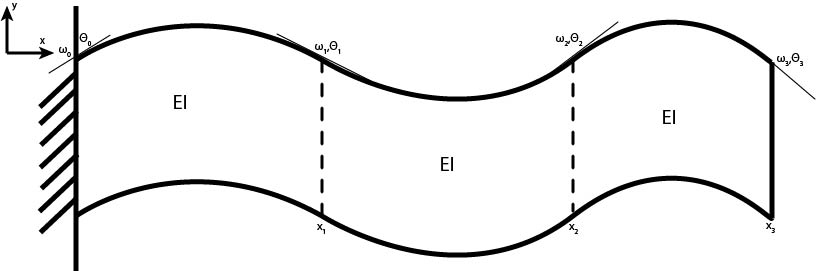
\includegraphics[width=.6\linewidth]{Figures/Beam.jpg}
\caption{Vibrating beam with states and stiffness labeled.}
\label{fig:Beam} 
\end{figure}
Extending this concept to a wing results in the configuration shown in Figure \ref{fig:CutWing}. The $Z_i$ and $\phi_{Z_i}$ are the states associated with spanwise bending which is defined as the vertical displacement along the spanwise axis. When speaking of a wing the spanwise direction is along the lateral axis. The states $X_i$ and $\phi_{X_i}$ are associated with the chordwise bending which is defined as the longitudinal displacement along the spanwise axis. The chord of a wing is the straight line connecting the leading and trailing edge of an airfoil, in Figure \ref{fig:CutWing} this is along the longitudinal axis. The final states shown are $\theta_i$ and $\phi_{\theta_i}$ which are the twist states of the wing about the lateral or spanwise axis. $n$ is the number of sections the wing is split into necessarily causing the number of sets of states to be $n+1$.
\begin{figure}[h]
\centering
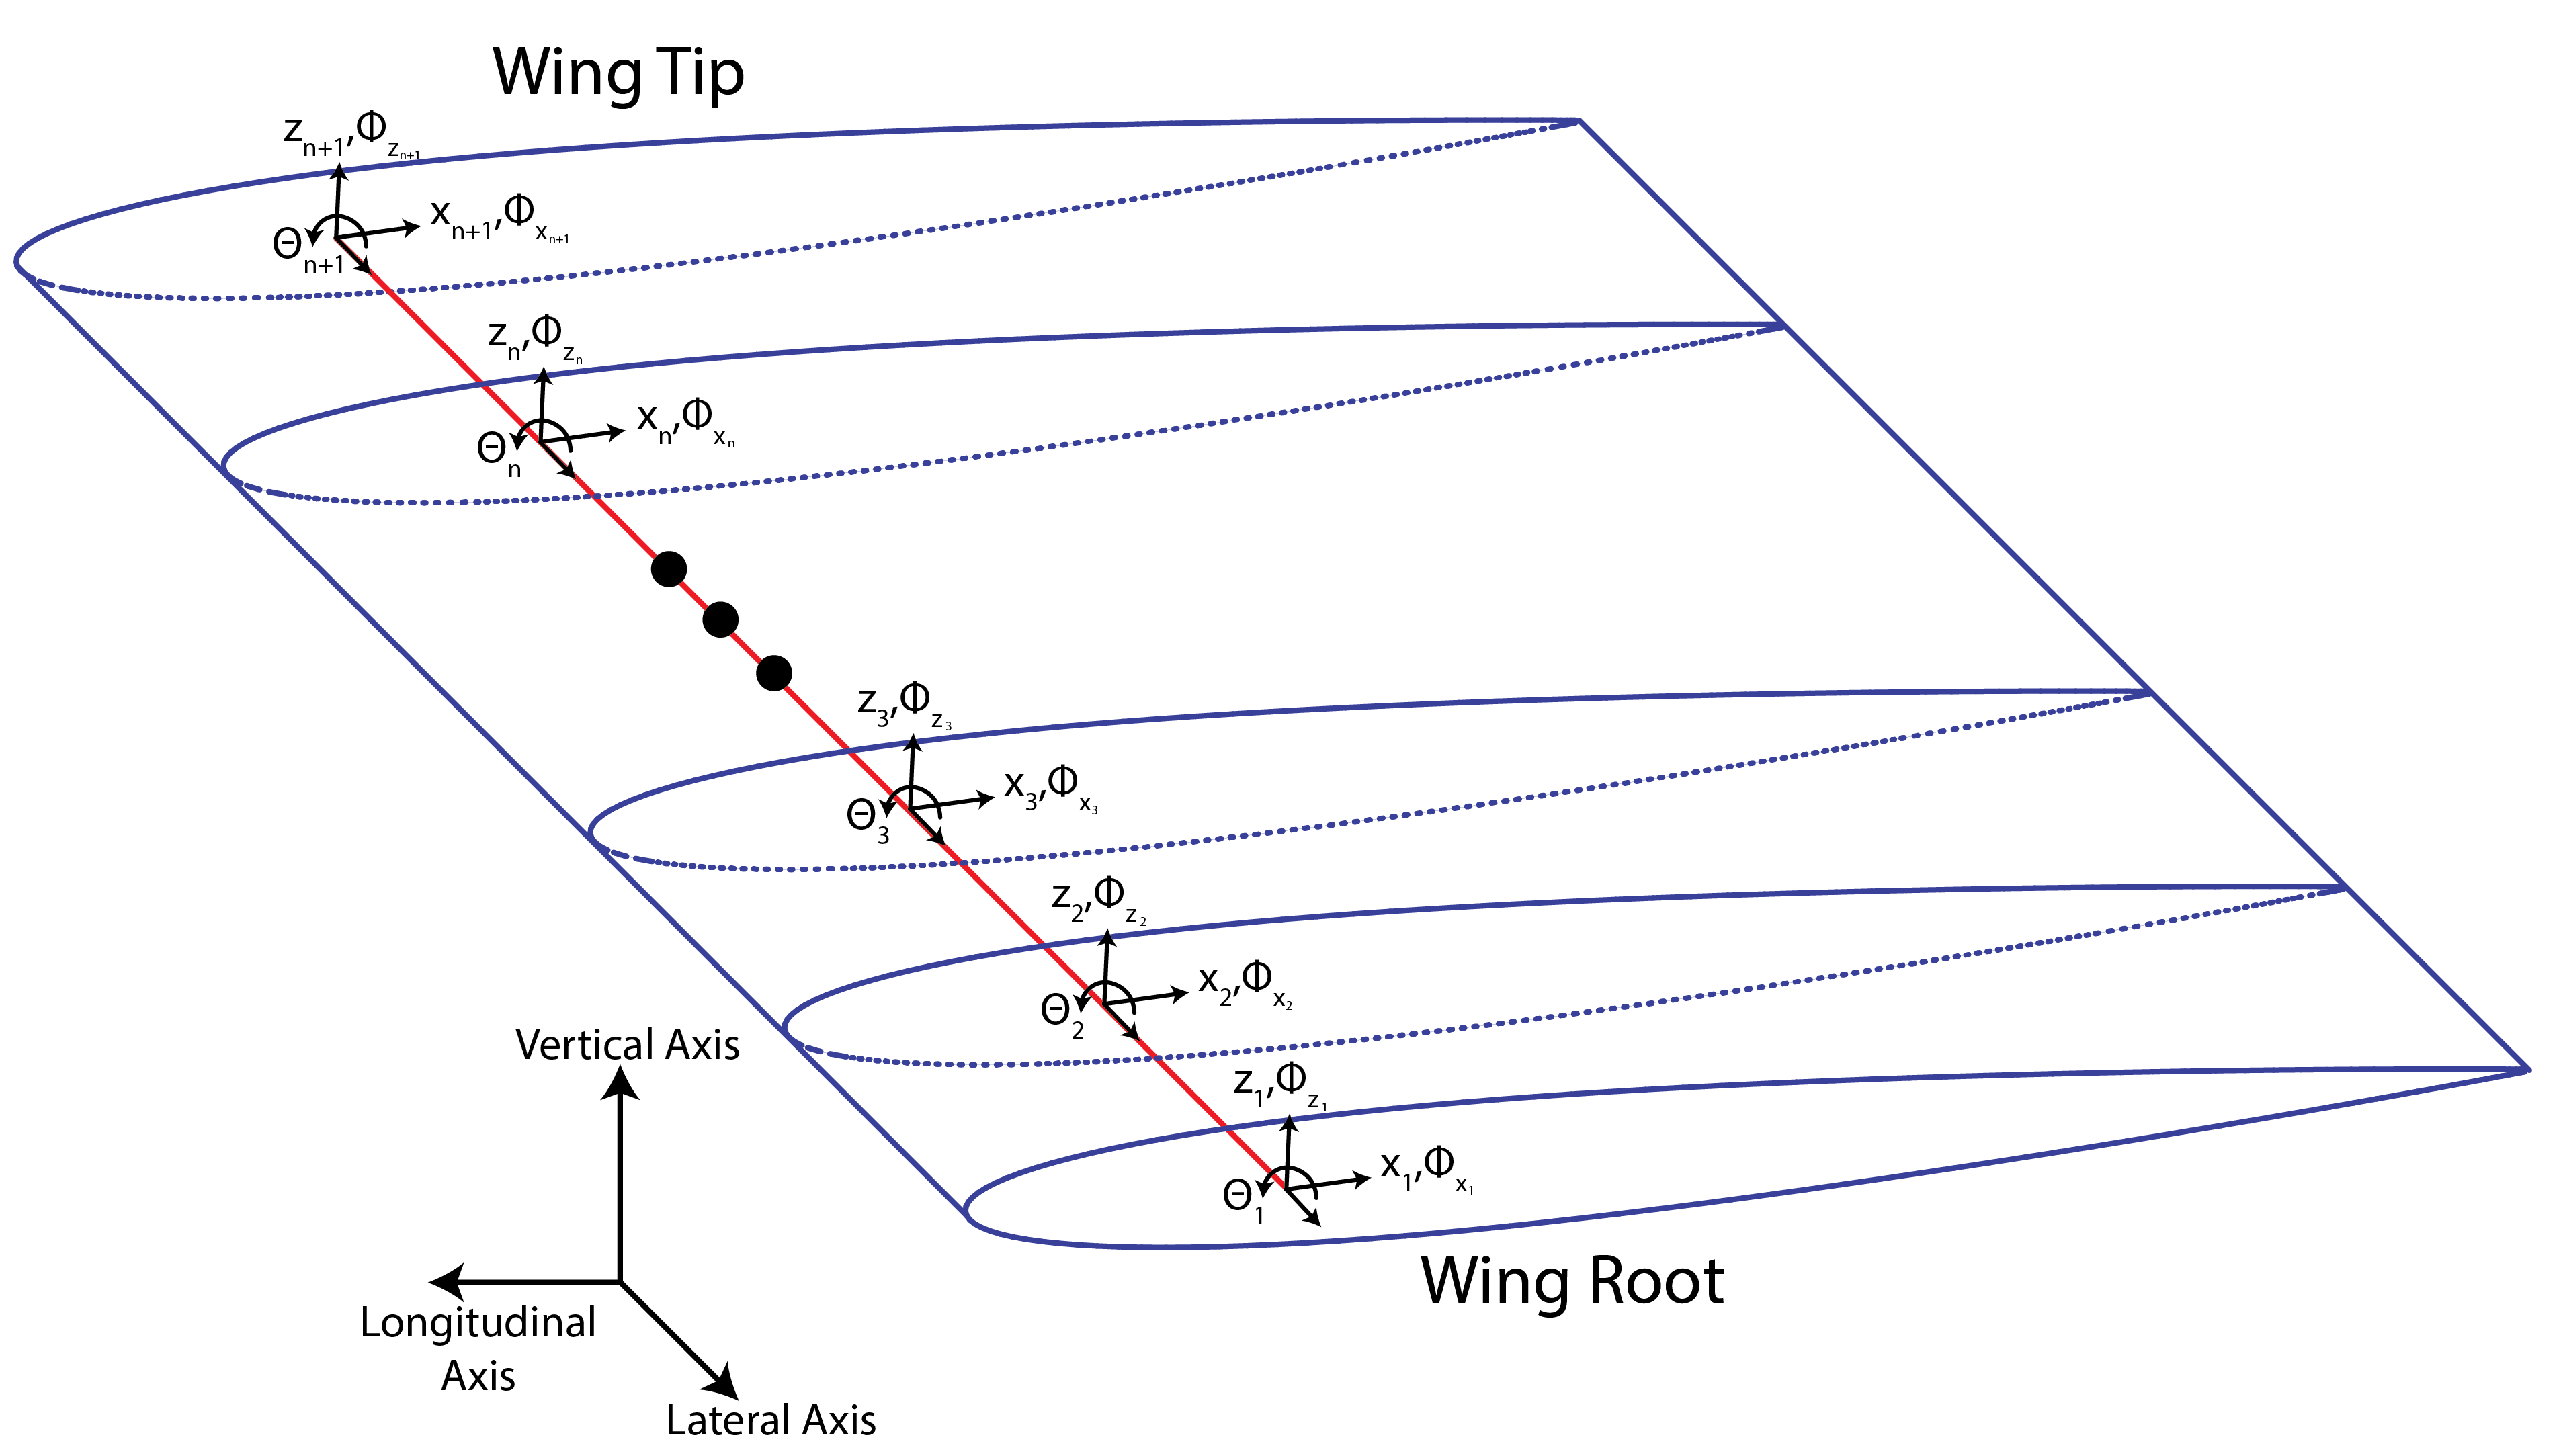
\includegraphics[width=1\linewidth]{Figures/StructuralWingStates-01.png}
\caption{Visualization of GFEM model of a wing with spanwise bending, chordwise bending and twist.}
\label{fig:CutWing} 
\end{figure}
This configuration has the dynamic equation presented in Equation \ref{eqn:GFEMeqn}
\begin{eqnarray}
X = [Z_1,\phi_{Z_1}, X_1,\phi_{X_1},\theta_1,\phi_{\theta_1}, \ldots,Z_{n+1},\phi_{Z_{n+1}}, X_{n+1},\phi_{X_{n+1}},\theta_{n+1},\phi_{\theta_{n+1}}]
\end{eqnarray}
\begin{eqnarray}
M\ddot{X}+C\dot{X}+KX = F
\label{eqn:GFEMeqn}
\end{eqnarray}
where going forward F can be populated by the aerodynamic forces.

\section{Aerodynamics}
In order to generate the aerodynamic forces that we generated by the wing we decided to use the standard vortex lattice method. The vortex lattice method (VLM) has some distinct advantages from other methods such as lifting line theory and traditional panel methods. VLM is capable of being used on any possible geometry unlike typical lifting line theory. It also includes the interaction in the spanwise direction unlike many of the traditional panel methods. VLM is also one of the more accurate methods for simulating aerodynamic lift. \cite{bertin1998aerodynamics} The biggest disadvantage to VLM is that it does not easily lend itself to viscid calculations. Given our expected application is a meso-scale UAV the viscid affects will likely not be an issue at the operating velocities.
\begin{figure}[h]
\centering
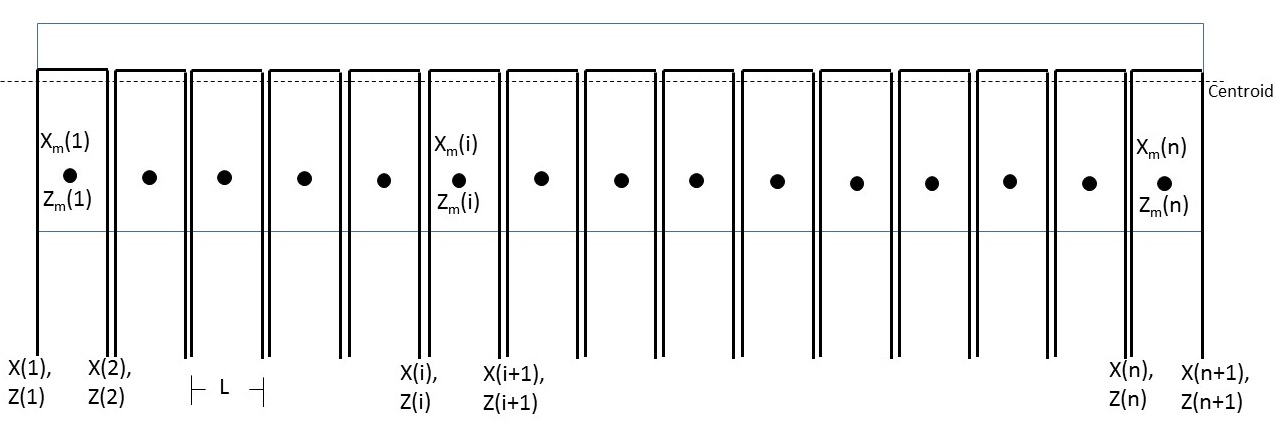
\includegraphics[width=1\linewidth]{Figures/VortexLaticeMethod.jpg}
\caption{VLM finite element horse shoe vortices with constant distances and centered about the three quarter cord line}
\label{fig:VLM}
\end{figure}

{\color{red}NOTE: ADD MOTIVATION FOR THE USE OF HORSESHOES INSTEAD OF RINGS HERE}

VLM uses finite elements in which horse shoe vortices are placed. These horse shoe vortices interactions is what creates the spanwise variation of the circulation about the wing. Figure \ref{fig:VLM} shows the set up for the VLM with the horse shoe vortices centered about the three quarter chord axis and the horizontal component of the horse shoe on the quarter chord axis. The horizontal vortex can be thought of as the circulation about the airfoil while the longitudinal vorticies are the trailing vortices that satisfy Helmholtz vortex theorem requiring that a bound-vortex does not change strength unless a separate vortex splits that is equal to the change in circulation. 

When comparing Figure \ref{fig:VLM} to Figure \ref{fig:CutWing} it can be seen how the VLM readily lends itself to the preexisting GFEM solid mechanics model. This was one of the reasons that the VLM was chosen to generate the aerodynamic forces, it has also already been shown to be a viable method for modeling aeroelastic effects in \cite{nguyencoupled,nguyen2012aeroelastic,nguyen2011longitudinal,nguyencoupled2014}.
\begin{figure}[h]
\centering
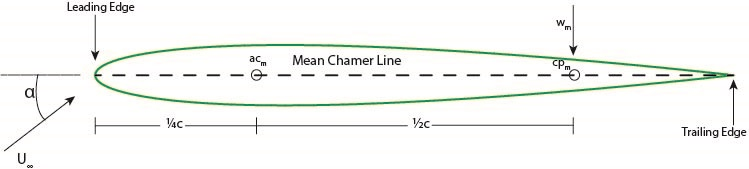
\includegraphics[width=1\linewidth]{Figures/AngleofAttack.jpg}
\caption{The angle of attack, $\alpha$, is the angle between the normal vector and the air velocity vector. For the symmetric airfoil the aerodynamic center is located at the quarter chord.}
\label{fig:alpha}
\end{figure}
While there are numerous prepackaged VLM softwares available we opted for writing a custom one primarily to have a base to build some of the proposed work that will be covered later. We based the VLM that we wrote off of the equations and methodology presented in \cite{bertin1998aerodynamics} with some auxiliary content taken from \cite{kundu2012fluid}. VLM uses Equation \ref{eqn:VLM} coupled with the boundary conditions provided in Equation \ref{eqn:VLMBC} to determine what the circulation about the airfoil is at a given control point $m$.
\begin{eqnarray}
\vec{V} = \vec{C}\Gamma_n
\label{eqn:VLM}
\end{eqnarray}
\begin{eqnarray}
-u_msin\delta cos\chi-v_mcos\delta sin\chi+w_mcos\chi cos\delta+U_{\infty}sin(\alpha-\delta)cos\chi = 0
\label{eqn:VLMBC}
\end{eqnarray}

where $\vec{V}$ is the generalized velocity vector at all the control points $m$, $\vec{C}$ is the geometry matrix that VLM generates from the current wing geometry, $\Gamma$ is the circulations at the control points. $u_m$, $v_m$, and $w_m$ are the local velocities at the control point $m$ in the longitudinal, lateral and vertical directions respectively. $U_{\infty}$ is the air speed, $\delta$ is the slope of the mean chamber line at the control point, $\chi$ is the dihedral angle, and $\alpha$ is the angle of attack. Figure \ref{fig:alpha} shows the mean chamber line which for a symmetric airfoil causes the slope of the mean chamber line, the $\delta$, to be equal to zero. Figure \ref{fig:alpha} also shows the angle of attack which is defined as $\frac{w_m}{U_{\infty}}$ where $w_m$ is the vertical induced velocity at the control point. Figure \ref{fig:dihedral} shows a wing from behind showing the dihedral angle.
\begin{figure}[h]
\centering
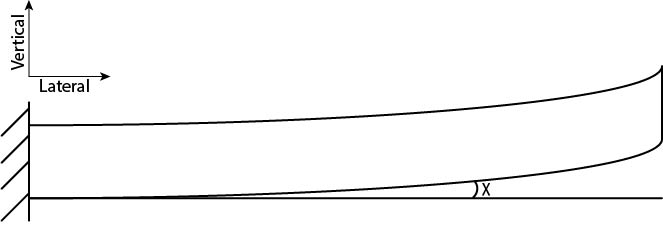
\includegraphics[width=0.5\linewidth]{Figures/DihedralAngle.jpg}
\caption{The dihedral angle is the angle between the spanwise slope of the wing and the wing root.}
\label{fig:dihedral}
\end{figure}

In order to combine and apply Equations \ref{eqn:VLM} and \ref{eqn:VLMBC} $\vec{C}$ needs to be generated. For each directional velocity in Equation \ref{eqn:VLMBC} a separate $\vec{C}$ can be generated by finding the velocity that each $\Gamma$ generated at a given control point. Each control point was chosen to be located at the three quarter chord and halfway between each spanwise GFEM element on the upper surface of the wing. Equations \ref{eqn:um}, \ref{eqn:vm}, \ref{eqn:wm} show how to populate the $m,n_{th}$ cell of matrix $\vec{C}$.
\begin{eqnarray}
	\begin{array}{ll}
		u_m = [(y_m-y_n)(z_m-z_{n+1})-(y_m-y_{n+1})(z_m-z_n)]/\\
		\{((y_m-y_n)(z_m-z_{n+1})-(y_m-y_{n+1})(z_m-z_n))^2\\
		+((x_m-x_n)(z_m-z_{n+1})-(x_m-x_{n+1})(z_m-z_n))^2\\
		+((x_m-x_n)(y_m-y_{n+1})-(x_m-x_{n+1})(y_m-y_n))^2\}
	\end{array}
\label{eqn:um}
\end{eqnarray}
\begin{eqnarray}
	\begin{array}{ll}
		v_m = -[(x_m-x_n)(z_m-z_{n+1})-(x_m-x_{n+1})(z_m-z_n)]/\\
		\{((y_m-y_n)(z_m-z_{n+1})-(y_m-y_{n+1})(z_m-z_n))^2\\
		+((x_m-x_n)(z_m-z_{n+1})-(x_m-x_{n+1})(z_m-z_n))^2\\
		+((x_m-x_n)(y_m-y_{n+1})-(x_m-x_{n+1})(y_m-y_n))^2\}\\
		+\frac{z_m-z_n}{4\pi((z_m-z_n)^2+(y_n-y_m)^2)}\left[1+\frac{x_m-x_n}{\sqrt{(x_m-x_n)^2+(y_m-y_n)^2+(z_m-z_n)^2}}\right]\\
		+\frac{z_m-z_{n+1}}{4\pi((z_m-z_{n+1})^2+(y_{n+1}-y_m)^2)}\left[1+\frac{x_m-x_{n+1}}{\sqrt{(x_m-x_{n+1})^2+(y_m-y_{n+1})^2+(z_m-z_{n+1})^2}}\right]
	\end{array}
\label{eqn:vm}
\end{eqnarray}
\begin{eqnarray}
	\begin{array}{ll}
		w_m = [(x_m-x_n)(y_m-y_{n+1})-(x_m-x_{n+1})(y_m-y_n)]/\\
		\{((y_m-y_n)(z_m-z_{n+1})-(y_m-y_{n+1})(z_m-z_n))^2\\
		+((x_m-x_n)(z_m-z_{n+1})-(x_m-x_{n+1})(z_m-z_n))^2\\
		+((x_m-x_n)(y_m-y_{n+1})-(x_m-x_{n+1})(y_m-y_n))^2\}\\
		+\frac{y_m-y_n}{4\pi((z_m-z_n)^2+(y_n-y_m)^2)}\left[1+\frac{x_m-x_n}{\sqrt{(x_m-x_n)^2+(y_m-y_n)^2+(z_m-z_n)^2}}\right]\\
		+\frac{y_m-y_{n+1}}{4\pi((z_m-z_{n+1})^2+(y_{n+1}-y_m)^2)}\left[1+\frac{x_m-x_{n+1}}{\sqrt{(x_m-x_{n+1})^2+(y_m-y_{n+1})^2+(z_m-z_{n+1})^2}}\right]
	\end{array}
\label{eqn:wm}
\end{eqnarray}

These equations represent the application of Biot-Savart law to the horse finite element horse shoes. The substitution of Equations \ref{eqn:um}, \ref{eqn:vm}, \ref{eqn:wm} into Equations \ref{eqn:VLM} and \ref{eqn:VLMBC} yield a system of equations that can be solve simultaneously by matrix inversion. 

{\color{red}NOTE: ADD INFORMATION ABOUT APPROXIMATION USED IN TORNADO}

\section{Aeroelastic}
Form a practical implementation perspective sense in the GFEM axial stretching and compressing were ignored all the components associated with $y$ are constant. The other variables $z$ and $x$ vary with the spanwise and chordwise deflections presented earlier. With the control points being placed between the GFEM states and allowing the edges of the horse shoe's to be placed on the GFEM states the amount of control points can be taken from $\lfloor \frac{2(n+1)}{5}\rfloor$ for having a control point and the edges of the horse shoe placed at GFEM states to $n$. The control point spanwise and chordwise deflections can be estimated with the cubic spline from Equation \ref{eqn:hCube} and then added to the initial geometric parameters of the wing to generate $z_m$ and $x_m$.

The exchange of position vectors between the solid mechanics and the aerodynamics does not represent the totality of the coupling in an aeroelastic system. Indeed the primary means of interaction between the two components if the aerodynamic forces that are applied to the wing. Utilizing the vortex lattice method we were able to generate the circulation at each control point. The circulation directly correspond to the lift and vortex induced drag forces as show in Equations \ref{eqn:liftF} and \ref{eqn:dragF}.
\begin{eqnarray}
l(y) = \rho_{\infty}U_{\infty}\Gamma(y)
\label{eqn:liftF}
\end{eqnarray}
\begin{eqnarray}
d(y) = tan(\theta(y)+\alpha_{root})l(y)
\label{eqn:dragF}
\end{eqnarray}
where $\theta$ is the twist of the wing at a given location $y$ and $\alpha_{root}$ is the angle of attack at the root of the wing. It is assumed that the air velocity is constant in the spanwise direction. Due to the fact that the control points are placed between GFEM states the force due to circulation does not directly apply to the state equation presented in \ref{eqn:GFEMeqn}. To address this we simply split the forces equally to each adjacent states. The generated force vector can then be put into Equation \ref{eqn:GFEMeqn} to complete the current iteration of this aeroelastic modeling.

The coupling of the aerodynamic states to the structural states allows for the creation of a static aeroelastic simulation tool, which is useful especially in the preliminary design and development stages but in some cases it is necessary to have a full dynamic aeroelastic model using an unsteady vortex lattice method. 

{\color{red} NOTE: IN THIS SECTION WE NEED TO GENERALIZE THESE EQUATIONS AND THE DEFINITIONS. MOST OF THIS CAN BE REGURGITATED IN THE LATER MORE RELEVANT SECTIONS}

In this study, we divide the digital wing into $m$ panels and calculate the aerodynamic forces/moments at each panel. Furthermore, we assume that the sectional element defined earlier coincides with the panel section, and we define $q$ collocation points around each panel section. We have chosen $q = 8$,and hence there are $mq = 128$ collocation points on each wing.     

\begin{figure}[h]
\centering
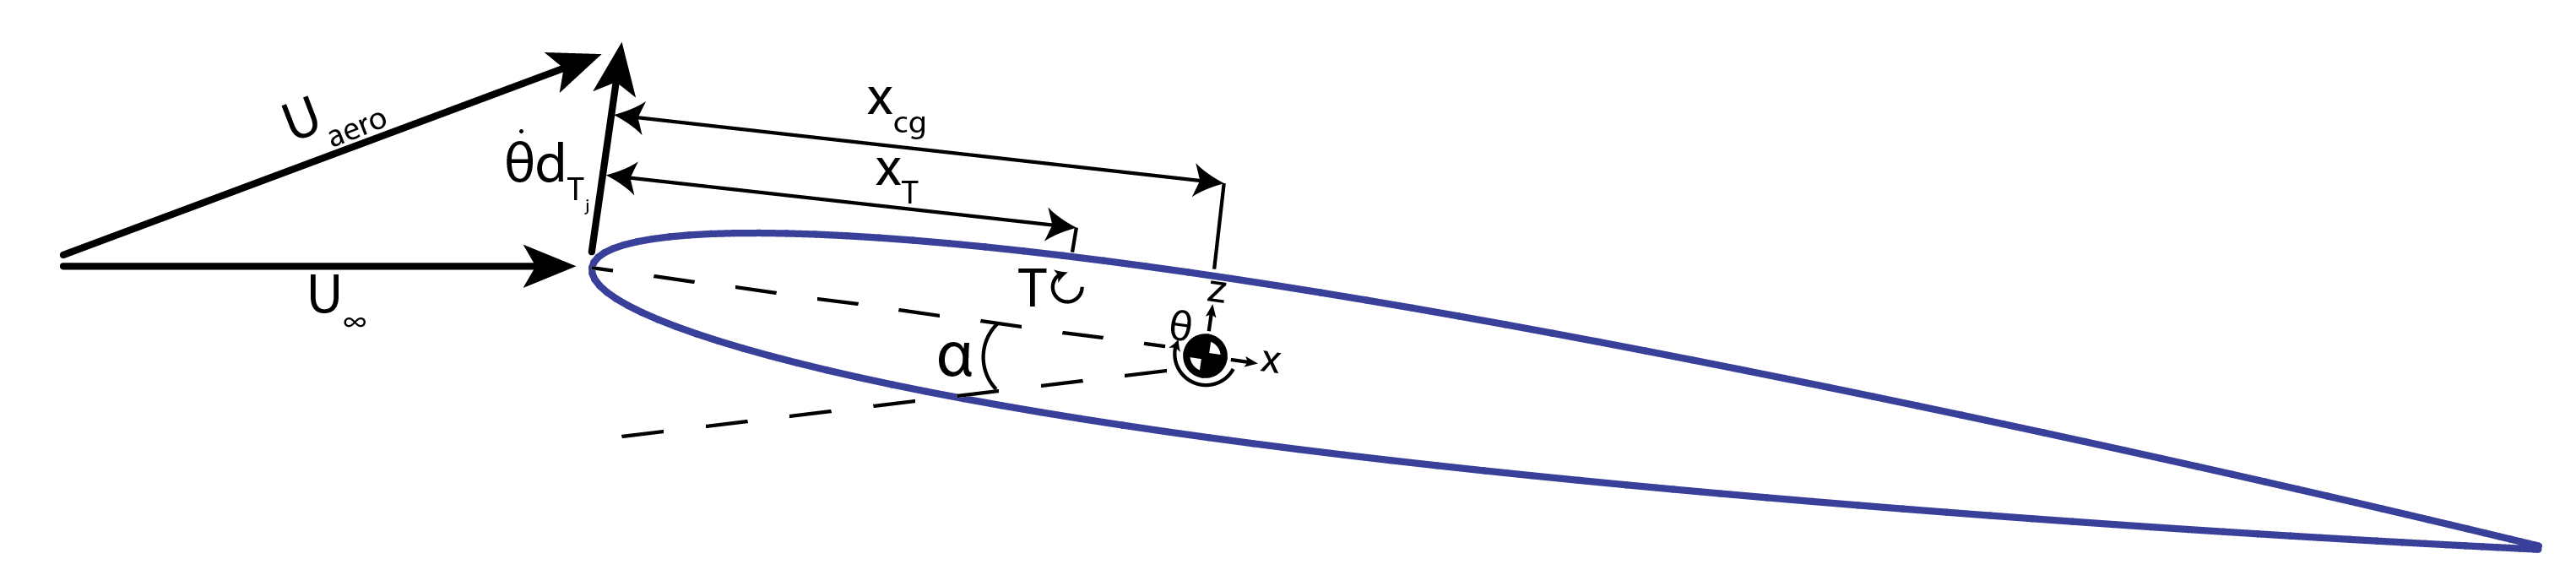
\includegraphics[width=1\linewidth]{Figures/AeroelasticDefinitions-01.png}
\caption{Aeroelastic definitions due to twist velocity}
\label{fig:def}
\end{figure}

The local aeroelastic wind velocity vector at each collocation point can be given by
\begin{equation}
U_{i,j} =\begin{bmatrix}U_{\infty} \;\; 0\end{bmatrix} R^T(\alpha_{root}) + \begin{bmatrix}\dot{\theta}_{i} |d_{j}| \;\; 0\end{bmatrix} R^T (\theta_{i}) \,,\;i=1,\cdots, m\,,\;j=1,\cdots, q
\label{eqn:Uinf}
\end{equation}
where $R(\cdot)$ denotes a $3\times 3$ rotational matrix, $\alpha_{root}$ is the angle of attack at the wing root, $U_{\infty}$ is the airspeed, $|d_{j}|$ is the magnitude of the position vector $d_{j}$ from torque tube axis to collocation point $j$, $\theta_i$ is the twist angle at $i$th panel, and $\dot{\theta}_i$ its rate. We should note that the local wind velocity $U_{i,j}$ defined in (\ref{eqn:Uinf}) is a tall matrix of dimension $mq \times 3$. To simplify the subsequent presentation, we rewrite its notation to be just $U_i$, where $i=1,\cdots,mq$. Then, the local aeroelastic angle of attack at each collocation point can be determined by
\begin{equation}
\alpha_{i} = \tan^{-1} \left (\frac{U_{iz}}{U_{ix}} \right) \,,\;i=1,\cdots, mq
\label{eqn:alpha_aero}
\end{equation}

Similarly, the local sideslip angle at section $i$, $\beta_i$, is given by 
\begin{equation}
\beta_{i} = \tan^{-1} \left (\frac{U_{iy}}{U_{ix}} \right) \,,\;i=1,\cdots, m
\label{eqn:beta_aero}
\end{equation}
where $U_{iy}$ is the $y$ component of $U_i$.

where $U_{ix}$ and $U_{iz}$ denote the $x$ and $z$ components of $U_{i}$. 

The circulation equation can be solved in its standard form as \cite{melin2000vortex}
\begin{equation}	\label{eqn:RHSGamma}
\left \{
\begin{array}{rll}
C_x \, \Gamma_x & = & B_x \\
C_y \, \Gamma_y & = & B_y \\
C_z \, \Gamma_z & = & B_z
\end{array}
\right .
\end{equation}
where $\Gamma_x$, $\Gamma_y$, and $\Gamma_z$ are the vectors of dimension $mq$ and denote the circulation of $mq$ collocation points in $(x,y,z)$ coordinates. The matrices $C_x$, $C_y$, and $C_z$ contain entries of influence coefficients that result form the geometry of the horseshoe vortex on collocation points in $(x,y,z)$ coordinates. The details on the influence coefficient matrix can be found in \cite{melin2000vortex}. Furthermore, the boundary conditions ${\bf B} = [B_x \;\; B_y \;\;B_z]$ are given by

\begin{equation}
{\bf B}_{i} = \begin{bmatrix}U_{ix}\cos(\alpha_{i})\cos(\beta)\\ -U_{iy}\cos(\alpha_{i})\sin(\beta)\\ U_{iz}\sin(\alpha_{i})\end{bmatrix}^T \,,\;i=1,\cdots,mq
\label{eqn:BC}
\end{equation}
where $\alpha_i$ is given in (\ref{eqn:alpha_aero}) and $\beta$ is the aircraft sideslip angle. Let ${\bf \Gamma} = [\Gamma_x \;\; \Gamma_y \;\;\Gamma_z]$, then we can solve for ${\bf \Gamma}_i$ by substituting (\ref{eqn:BC}) into (\ref{eqn:RHSGamma}). Therefore, the total aerodynamic forces and moments on the digital wing can be derived from each panel as %given collocation points can be solved by
\begin{equation}
% \begin{array}{l}
F = \rho_{\infty} \sum_{i=1}^{mq} ({\bf B}_i \otimes {\bf \Gamma}_i)
\label{eqn:aeroForce}
\end{equation}
and
\begin{equation}
M = \rho_{\infty} \left [ \sum_{i=1}^{mq} (d_i-m_c) \otimes ({\bf B}_i \otimes {\bf \Gamma}_i)\,\right ]
\label{eqn:aeroMoment}
\end{equation}
where $\rho_{\infty}$ is the air density, $d_i$ the $i$th collocation point position vector, $m_c$ the position vector to the center of gravity, and $\otimes$ denotes the vector cross product. It should be noted that the sectional aerodynamic forces and moments from (\ref{eqn:aeroForce}) and (\ref{eqn:aeroMoment}) are coupled with the structural dynamics described in (\ref{eqn:SEoM}). Finally, the total aerodynamic lift ($L$), drag ($D$), and lateral force ($S$) can be given by 
\begin{equation}
\begin{bmatrix}D\\S\\L\end{bmatrix} = R(\alpha_{root})R(\beta)\begin{bmatrix}F_{ax}\\F_{ay}\\F_{az}\end{bmatrix}
\label{eqn:LDS}
\end{equation}
where $F = [F_{ax} \;\;F_{ay} \;\; F_{az}]^{T}$.   

%%%%%%%%%%%%%%%%%%%%%%%%%%%%%%%%%%%%%%%%%%%%%%%%%%%%%%%%%%%%%%%%%%%%%%%%%%%
\chapter{Preliminary Modeling and Design}

%%%%%%%%%%%%%%%%%%%%%%%%%%%%%%%%%%%%%%%%%%%%%%%%%%%%%%%%%%%%%%%%%%%%%%%%%%%
\chapter{Testing and Validation}
\section{Wind Tunnel Testing}
\section{Results and Validation}

%%%%%%%%%%%%%%%%%%%%%%%%%%%%%%%%%%%%%%%%%%%%%%%%%%%%%%%%%%%%%%%%%%%%%%%%%%%
\chapter{Control}
\section{Structural Stability Control of Lattice Structure}
\subsection{Structural Decentralized Control}
\subsection{Transfer Matrix Method}

\section{Active Twist Aircraft Control}

%%%%%%%%%%%%%%%%%%%%%%%%%%%%%%%%%%%%%%%%%%%%%%%%%%%%%%%%%%%%%%%%%%%%%%%%%%%
\chapter{Conclusion}
\section{Summary}
\section{Future Works}

\nocite{*}
\bibliographystyle{plain}
\bibliography{thesis}

\end{document}
